
\documentclass[english,notitlepage]{revtex4-1}  % defines the basic parameters of the document
%For preview: skriv i terminal: latexmk -pdf -pvc filnavn



% if you want a single-column, remove reprint

% allows special characters (including æøå)
\usepackage[utf8]{inputenc}
%\usepackage[english]{babel}

%% note that you may need to download some of these packages manually, it depends on your setup.
%% I recommend downloading TeXMaker, because it includes a large library of the most common packages.

\usepackage{physics,amssymb}  % mathematical symbols (physics imports amsmath)
\include{amsmath}
\usepackage{graphicx}         % include graphics such as plots
\usepackage{xcolor}           % set colors
\usepackage{hyperref}         % automagic cross-referencing (this is GODLIKE)
\usepackage{listings}         % display code
\usepackage{subfigure}        % imports a lot of cool and useful figure commands
\usepackage{float}
%\usepackage[section]{placeins}
\usepackage{algorithm}
\usepackage[noend]{algpseudocode}
\usepackage{subfigure}
\usepackage{tikz}
\usetikzlibrary{quantikz}
% defines the color of hyperref objects
% Blending two colors:  blue!80!black  =  80% blue and 20% black
\hypersetup{ % this is just my personal choice, feel free to change things
    colorlinks,
    linkcolor={red!50!black},
    citecolor={blue!50!black},
    urlcolor={blue!80!black}}

%% Defines the style of the programming listing
%% This is actually my personal template, go ahead and change stuff if you want



%% USEFUL LINKS:
%%
%%   UiO LaTeX guides:        https://www.mn.uio.no/ifi/tjenester/it/hjelp/latex/
%%   mathematics:             https://en.wikibooks.org/wiki/LaTeX/Mathematics

%%   PHYSICS !                https://mirror.hmc.edu/ctan/macros/latex/contrib/physics/physics.pdf

%%   the basics of Tikz:       https://en.wikibooks.org/wiki/LaTeX/PGF/Tikz
%%   all the colors!:          https://en.wikibooks.org/wiki/LaTeX/Colors
%%   how to draw tables:       https://en.wikibooks.org/wiki/LaTeX/Tables
%%   code listing styles:      https://en.wikibooks.org/wiki/LaTeX/Source_Code_Listings
%%   \includegraphics          https://en.wikibooks.org/wiki/LaTeX/Importing_Graphics
%%   learn more about figures  https://en.wikibooks.org/wiki/LaTeX/Floats,_Figures_and_Captions
%%   automagic bibliography:   https://en.wikibooks.org/wiki/LaTeX/Bibliography_Management  (this one is kinda difficult the first time)
%%   REVTeX Guide:             http://www.physics.csbsju.edu/370/papers/Journal_Style_Manuals/auguide4-1.pdf
%%
%%   (this document is of class "revtex4-1", the REVTeX Guide explains how the class works)


%% CREATING THE .pdf FILE USING LINUX IN THE TERMINAL
%%
%% [terminal]$ pdflatex template.tex
%%
%% Run the command twice, always.
%% If you want to use \footnote, you need to run these commands (IN THIS SPECIFIC ORDER)
%%
%% [terminal]$ pdflatex template.tex
%% [terminal]$ bibtex template
%% [terminal]$ pdflatex template.tex
%% [terminal]$ pdflatex template.tex
%%
%% Don't ask me why, I don't know.

\begin{document}

\title{Project 1 - FYS3150}      % self-explanatory
\author{Dag Arne Lydvo}          % self-explanatory
\date{\today}                             % self-explanatory
\noaffiliation                            % ignore this, but keep it.


\maketitle 
    
\textit{List a link to your github repository here!}
    
\section*{Problem 1}

\[-\frac{d^2u}{dx^2}=f(x)=100e^{-10x} \]
Solving for u:
\[-u = \int\int 100e^{-10x} dx^2\]
Using $w = -10x$ and $dx=\frac{dw}{-10}$
\[-u = 100\int\int e^{w}\frac{dw^2}{-10}\]
\[ -u = -10 \int e^{-10x}+C_1 dx\]
\[-10\int e^w +C_1 \frac{dw}{-10} = e^w + C_1w + C_2\]
\[-u = e^{-10x} +C_1(-10x)+C_2\]
Solving for constants using boundary conditions $u(0)=u(1)=0$
\[-u(0)=0=e^0 +C_2 \rightarrow C_2=-1\]
\[-u(1)=0=e^{-10}+C_1(-10)-1 \rightarrow C_1=\frac{1}{10}(e^{-10}-1)\]
\[-u(x) = e^{-10x}+\frac{1}{10}(e^{-10}-1)(-10x)-1\]
\[u(x)=1-(1-e^{-10})x - e^{-10x}\]
\section*{Problem 2}
\begin{figure}
	\centering
	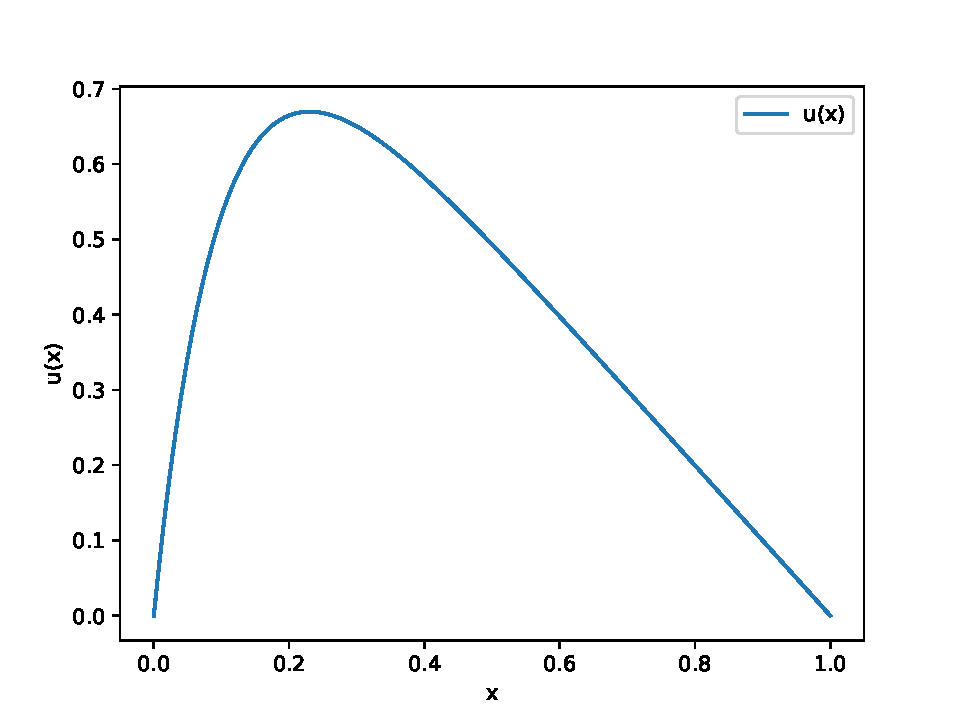
\includegraphics[scale=0.75]{../Figures/problem_2.pdf}
	\caption{Exact solution of u(x) over 1000 steps of x.}
\end{figure}




\section{Problem 3}
\[-\frac{d^2u}{dx^2}=f(x)\]

The continous variable x becomes discrete, $x\rightarrow x_1$\\
Where i = (0,1,...,n), where n is the number of steps. 

$u(x)$ becomes $u(x_i)$, and $u(x_1)=u(x_0+h)$,
where h is the step size defined as $ h = \frac{x_n-x_0}{n}$

The discrete version of $-\frac{d^2u}{dx^2}= f(x)$ now becomes \

\[ -\frac{d^2u}{dx^2} \vert_{x_i}= \frac{u_{i+1} + u_{i-1} - 2u_i}{h^2} + O(h^2) \]

and the approximation can be written as 
\[v''_i = \frac{-v_{i+1}-v_{i-1}+2v_i}{h^2} = f_i\]


\section{Problem 4}

The approximte discrete version of the Poisson equation from problem 3 can be rewritten as \[-v_{i+1}-v_{i-1}+2v_i = f_i h\]

Here we have n numbers of unknown variables $v_i$ for $i=(0,1,...,n)$ making up the the vector $\vec{v}=(v_0,v_1,...,v_n)$. We also have n numbers of known functions $g_i = f_i h^2$ making up the vector $\vec{g}=(f_0,f_1,...,f_n)$. 

The termns of $v'' h^2 = v_{i-1}-2v_i+v_{i+1}$ makes up  n sets of equations. 

\[2v_1- v_2 = g_1\]
\[-v_1 + 2v_2 - v_3 = g_2\]
 \[ .  .  . \]
  \[.  .  . \]
  \[.  .  . \]
\[-v_{n-1} + 2v_n = g_n\]

The terms of $-v_0 and -v_n+1$ are zero because of the boundary conditions. The first and last equations therefore contains only two terms. 

This set of equations can then be written as the matrix equation $\vb{A}\vec{v} = \vec{g}$. \\
Where $\vb{A}$ is:
\[
\begin{bmatrix}
 2  & -1 & 0 &\dots & 0 \\
 -1 & 2  & -1 & \dots & 0 \\
 \vdots & \vdots & \ddots &\dots & 0 \\
 0 & 0 &-1 & 2 & -1 \\
 0 & 0 & 0& -1 & 2 & 
\end{bmatrix} \]\\
and $\vec{v}$ and $ \vec{g}$ is: 
\[\begin{bmatrix}
	v_1 \\ v_2 \\ \vdots \\ v_n
\end{bmatrix}\begin{bmatrix}
	g_1 \\ g_2 \\ \vdots \\ g_n
\end{bmatrix}\]


\section{Problem 5}

\section{Problem 6}
Solving a general tridiagonal matrix can be done by two general steps. First forward substitution then backward substitution on the subdiagonal $a_i$, main diagonal $b_i$ and superdiagonal $c_i$.  
\begin{algorithm}[H]
	\caption{Solving general tridiagonal matrix}\label{algo:midpoint_rule}
	\begin{algorithmic}
		\State Forward substitution
		\State $\tilde{b_0}=b_0$  \Comment{Here's a comment}
		\State $\tilde{g_0}=g_0$
		\For{$i =  1, ..., n$}
		\State $\tilde{b_i} = b_i - \frac{a_i}{\tilde{b_{i-1}}}c_{i-1}$ \Comment{3(n-1) FLOPs}
		\State $\tilde{g_i} = g_i - \frac{a_i}{\tilde{b_{i-1}}}\tilde{g_{i-1}}$ \Comment{3(n-1) FLOPs}
		\EndFor
		
		\State Backward substitution 
		\State $v_n = \frac{\tilde{g_n}}{\tilde{b_n}}$ \Comment{1 FLOP}
		\For{$i = n-1,n-2, ...,1}$
		\State $v_i = \frac{\tilde{g_i}-c_iv_{i+1}}{\tilde{b_i}}$ \Comment{3(n-1) FLOPs}
		\EndFor
		
	\end{algorithmic}
\end{algorithm}

With the forward subs. not counting the first element $i=0$ and the backward substitution not counting the last element $i=n$ both for loops runs for $n-1$ loops. 
The total FLOPs for the algorithm then becomes $9(n-1) + 1$


\section{Problem 7}
\begin{figure}
	\centering
	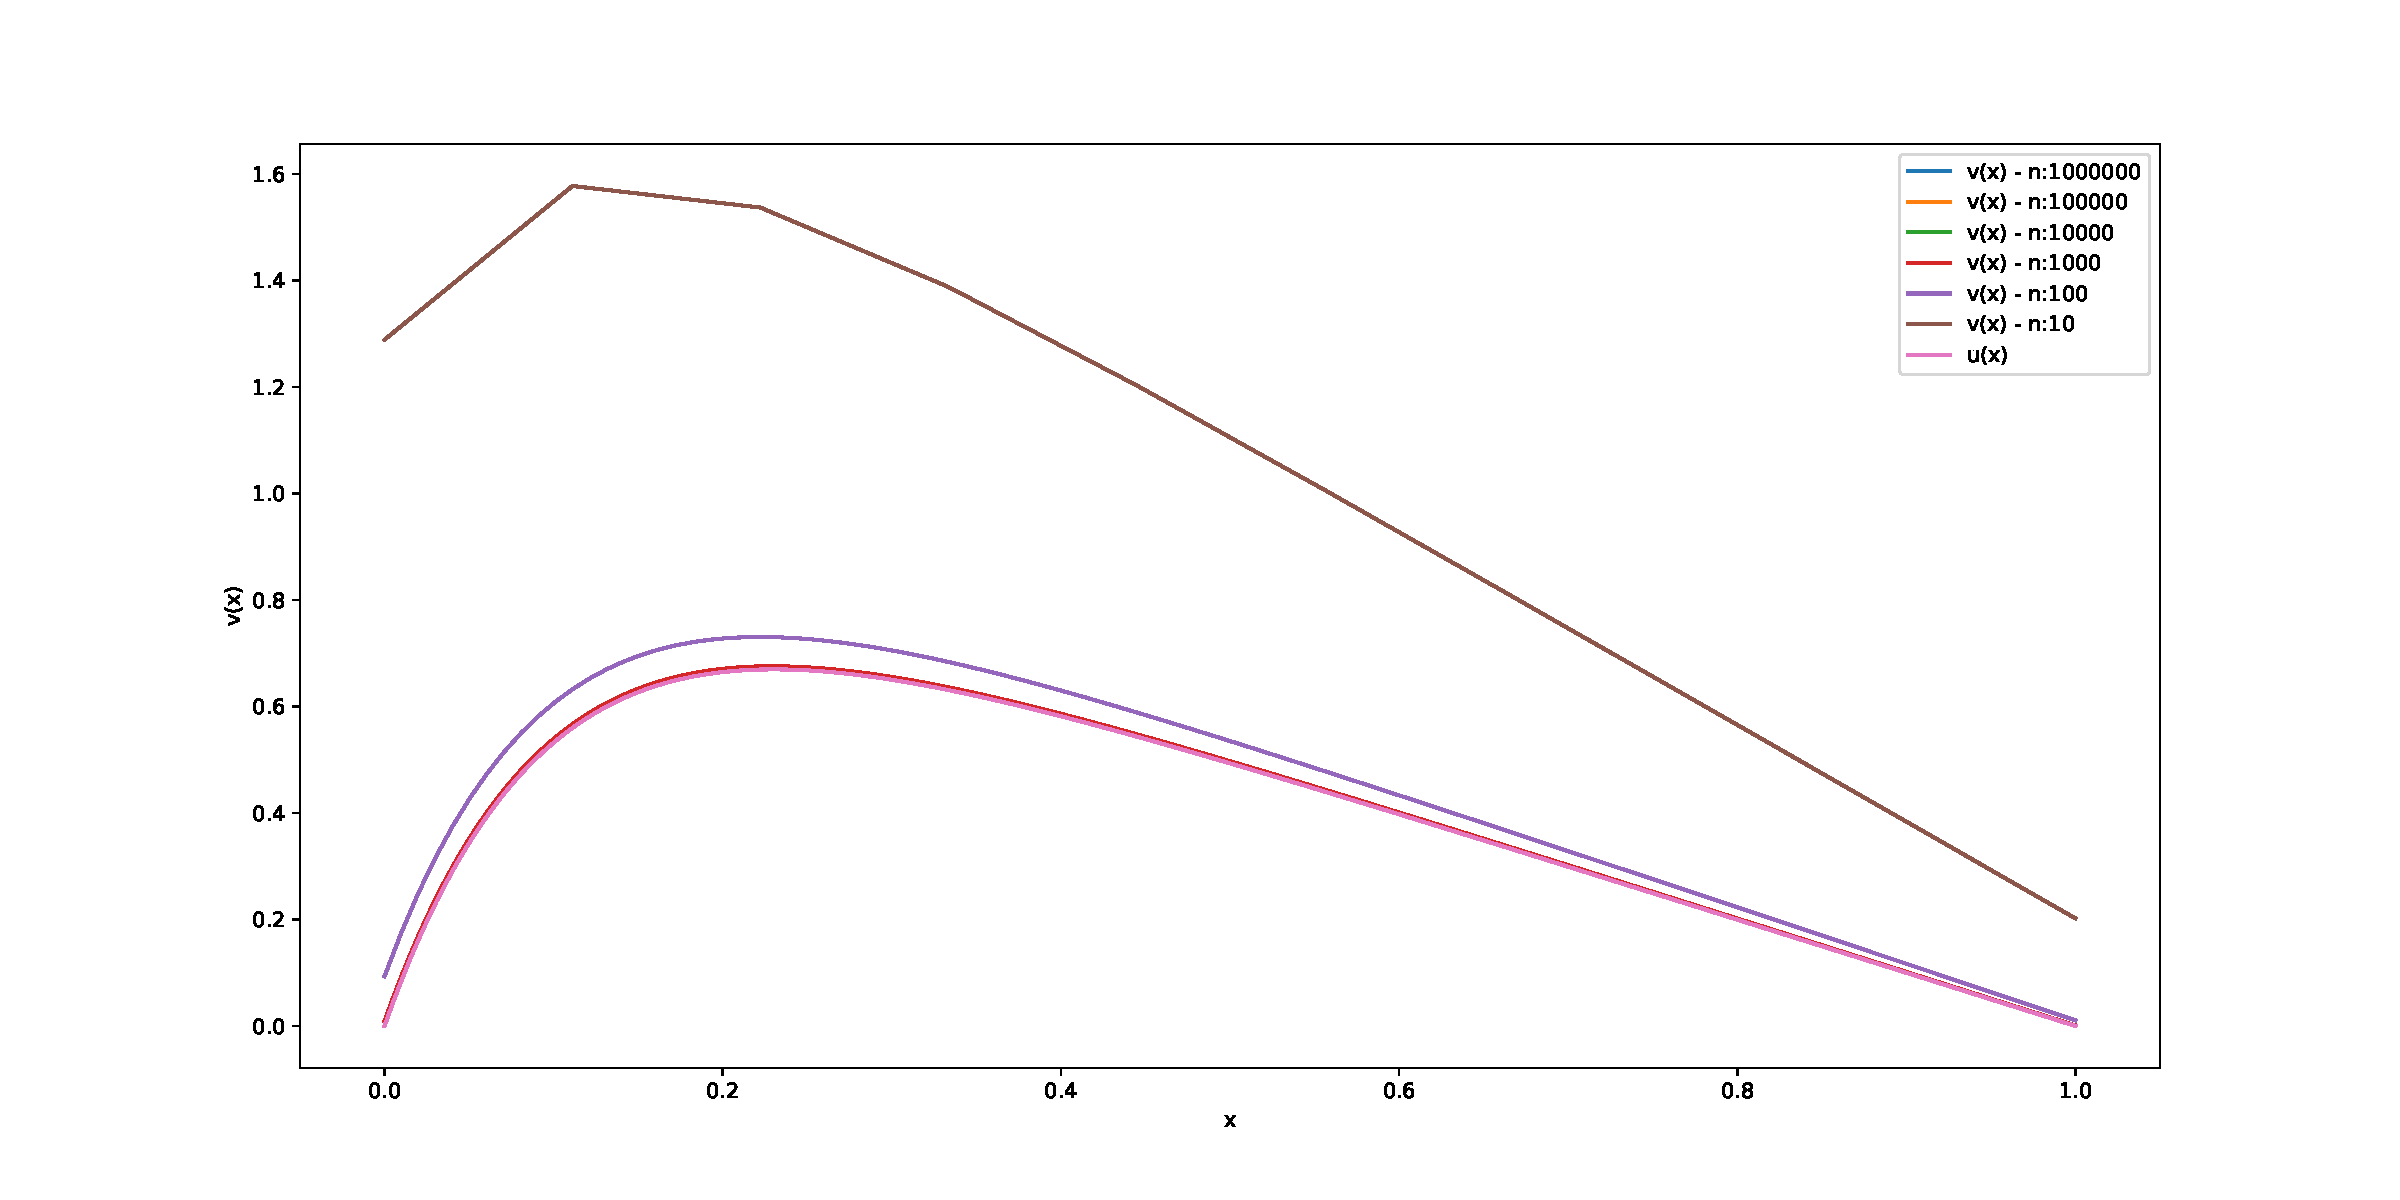
\includegraphics[scale=0.5]{../Figures/problem7.pdf}
	\caption{Numerical solution using the general algorithm with varying values of n vs the exact solution u(x)}
\end{figure}

\section{Problem 8}

\begin{figure}
	\centering
	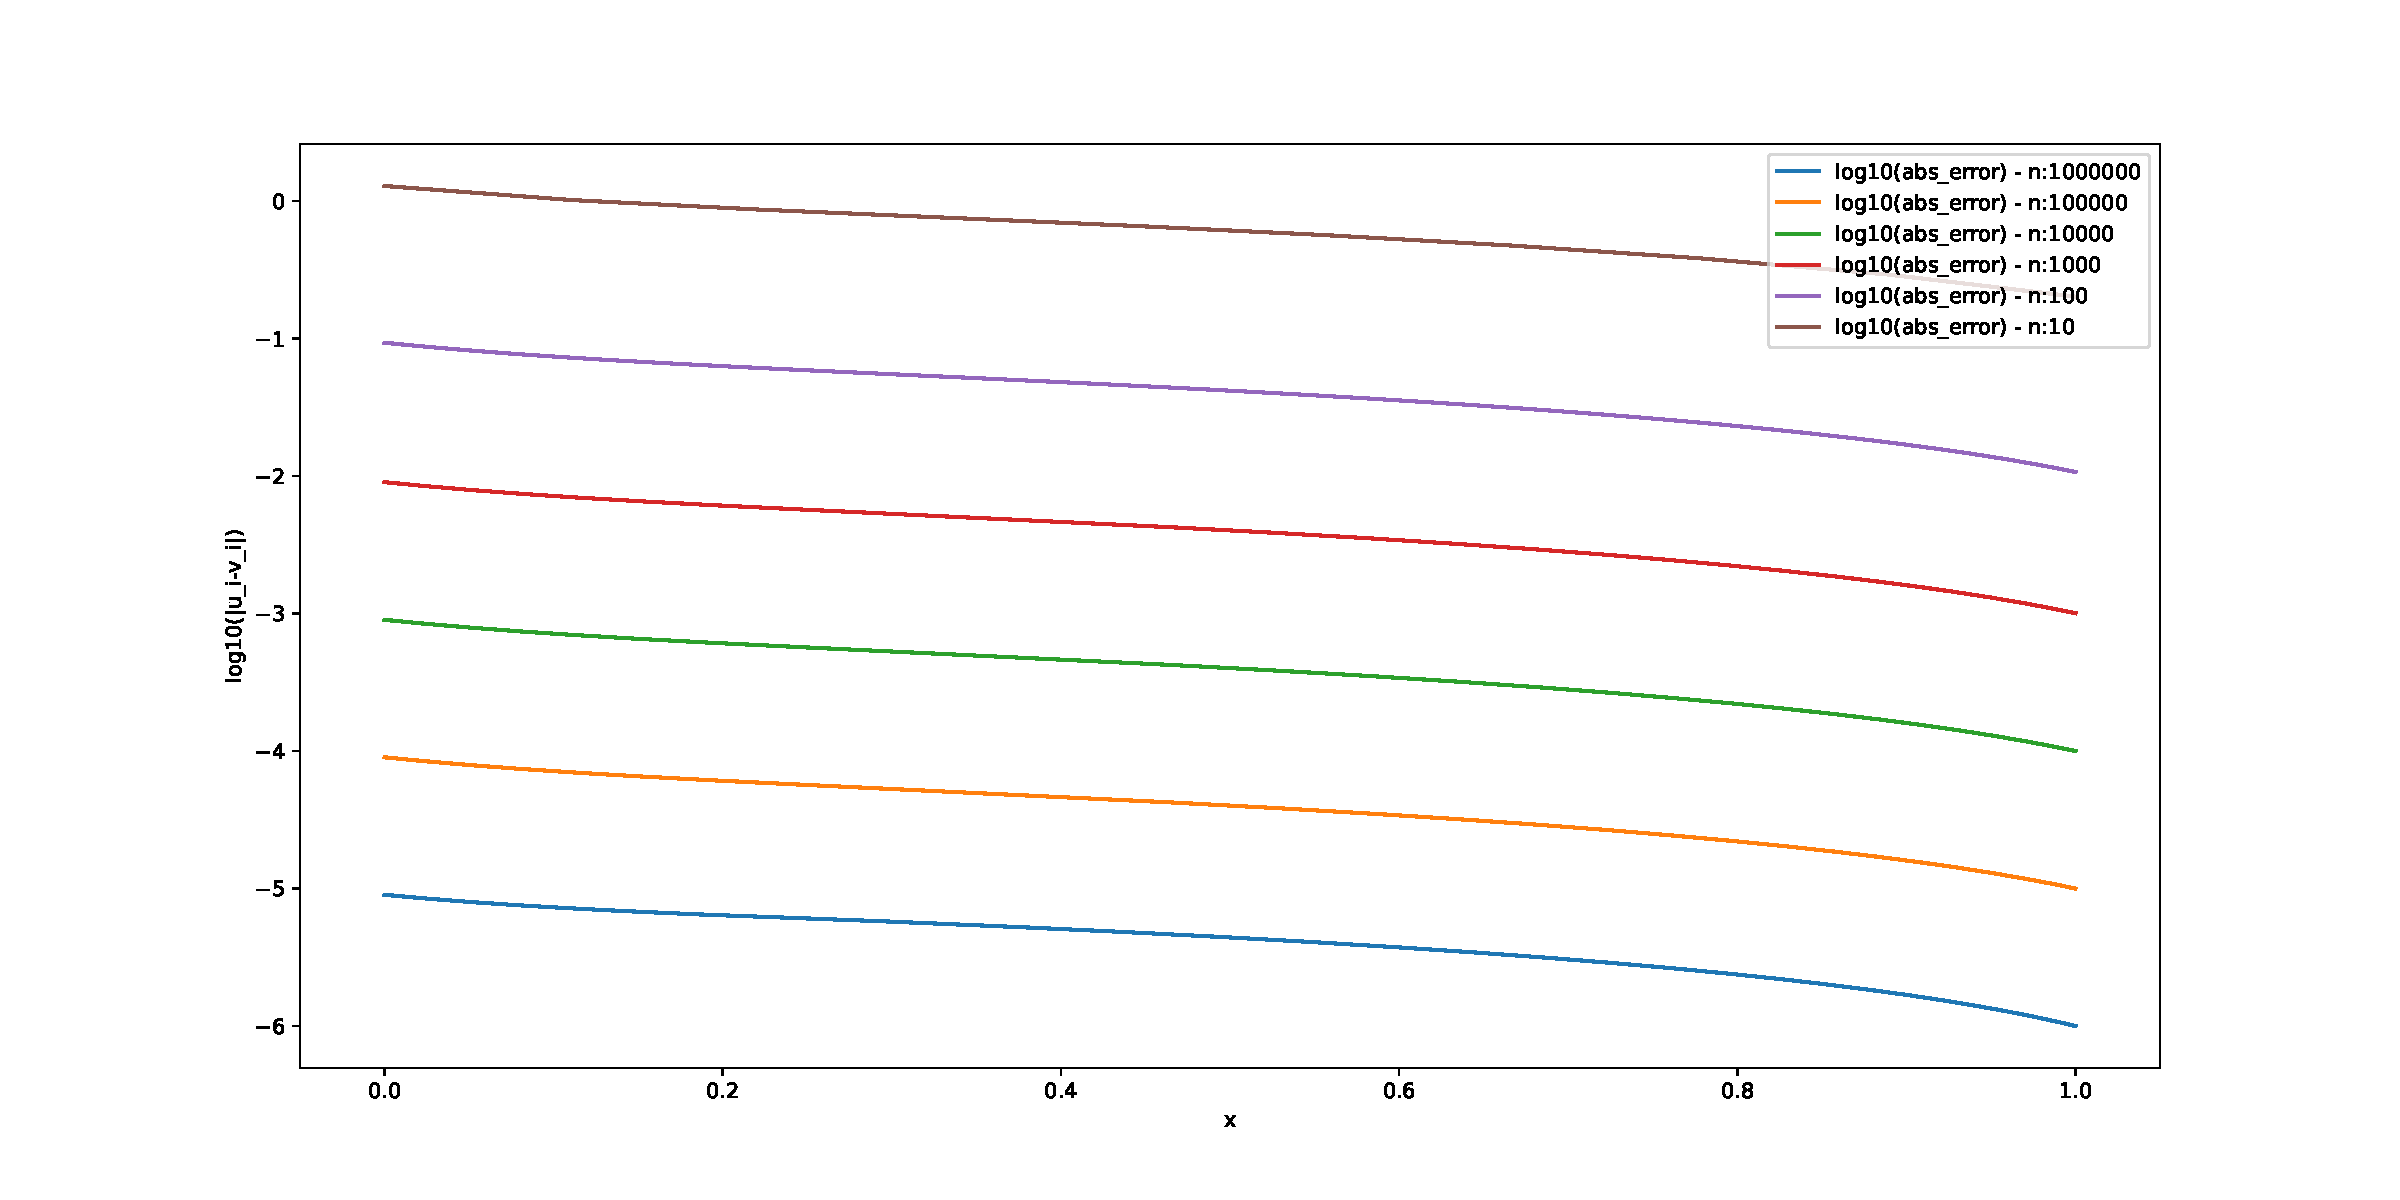
\includegraphics[scale=0.5]{../Figures/problem8_abs_error.pdf}
	\caption{Numerical solution using the general algorithm with varying values of n vs the exact solution u(x)}
\end{figure}
\begin{figure}
	\centering
	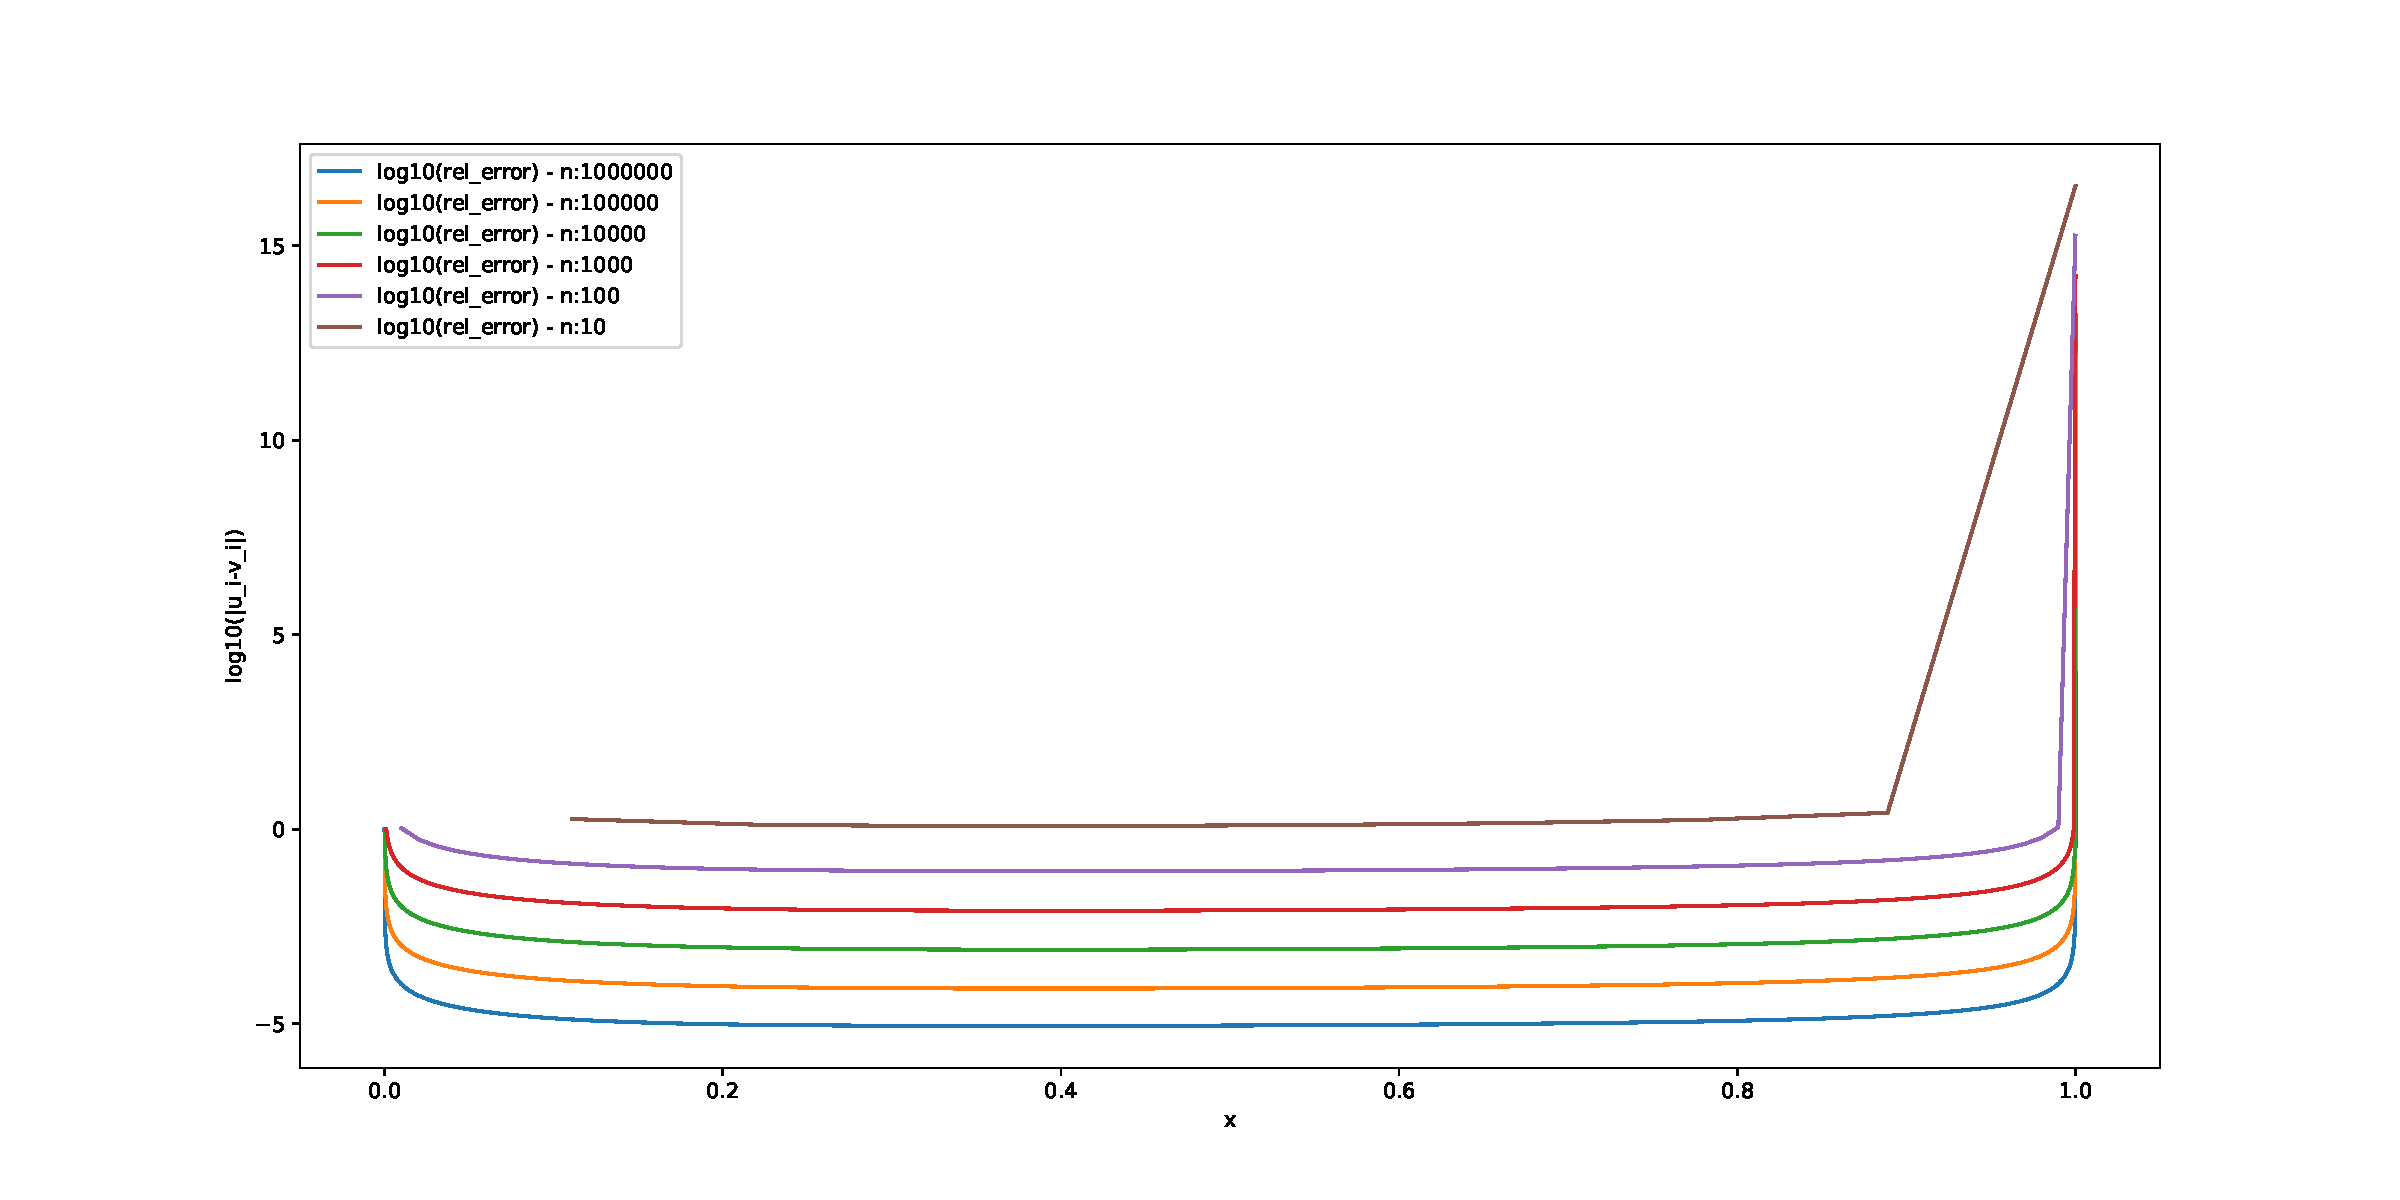
\includegraphics[scale=0.5]{../Figures/problem8_rel_error.pdf}
	\caption{Numerical solution using the general algorithm with varying values of n vs the exact solution u(x)}
\end{figure}
\begin{figure}
	\centering
	\includegraphics[scale=1]{../Figures/problem8_table.pdf}
	\caption{Numerical solution using the general algorithm with varying values of n vs the exact solution u(x)}
\end{figure}



\section[h]{Problem 9}

For the special case where the matrix $\vb{A}$ as a signature of (-1,2,-1), the diagonal vectors have constant values the general algorithm will be modified to possible reduce the number of FLOPs.
 
Since the values for $a_i$ and $c_i$ are constant the operations between these values can be removed. And since the value of $a$ and $c$ are $-1$ we can just switch the operator.
This special algorithm reduces the number of FLOPs from $9(n-1)+1$ to $6(n-1)+1$. 
\begin{algorithm}[H]
	\caption{Solving special tridiagonal matrix}\label{algo:midpoint_rule}
	\begin{algorithmic}
		\State Forward substitution
		\State $\tilde{b_0}=b_0$  \Comment{Here's a comment}
		\State $\tilde{g_0}=g_0$
		\For{$i =  1, ..., n$}
		\State $\tilde{b_i} = b_i - \frac{1}{\tilde{b_{i-1}}}$ \Comment{2(n-1) FLOPs}
		\State $\tilde{g_i} = g_i + \frac{\tilde{g_{i-1}}}{\tilde{b_{i-1}}}$ \Comment{2(n-1) FLOPs}
		\EndFor
		
		\State Backward substitution 
		\State $v_n = \frac{\tilde{g_n}}{\tilde{b_n}}$ \Comment{1 FLOP}
		\For{$i = n-1,n-2, ...,1}$
		\State $v_i = \frac{\tilde{g_i}+v_{i+1}}{\tilde{b_i}}$ \Comment{2(n-1) FLOPs}
		\EndFor
		
	\end{algorithmic}
\end{algorithm}


\section{Problem 10}
\begin{figure}
	\centering
	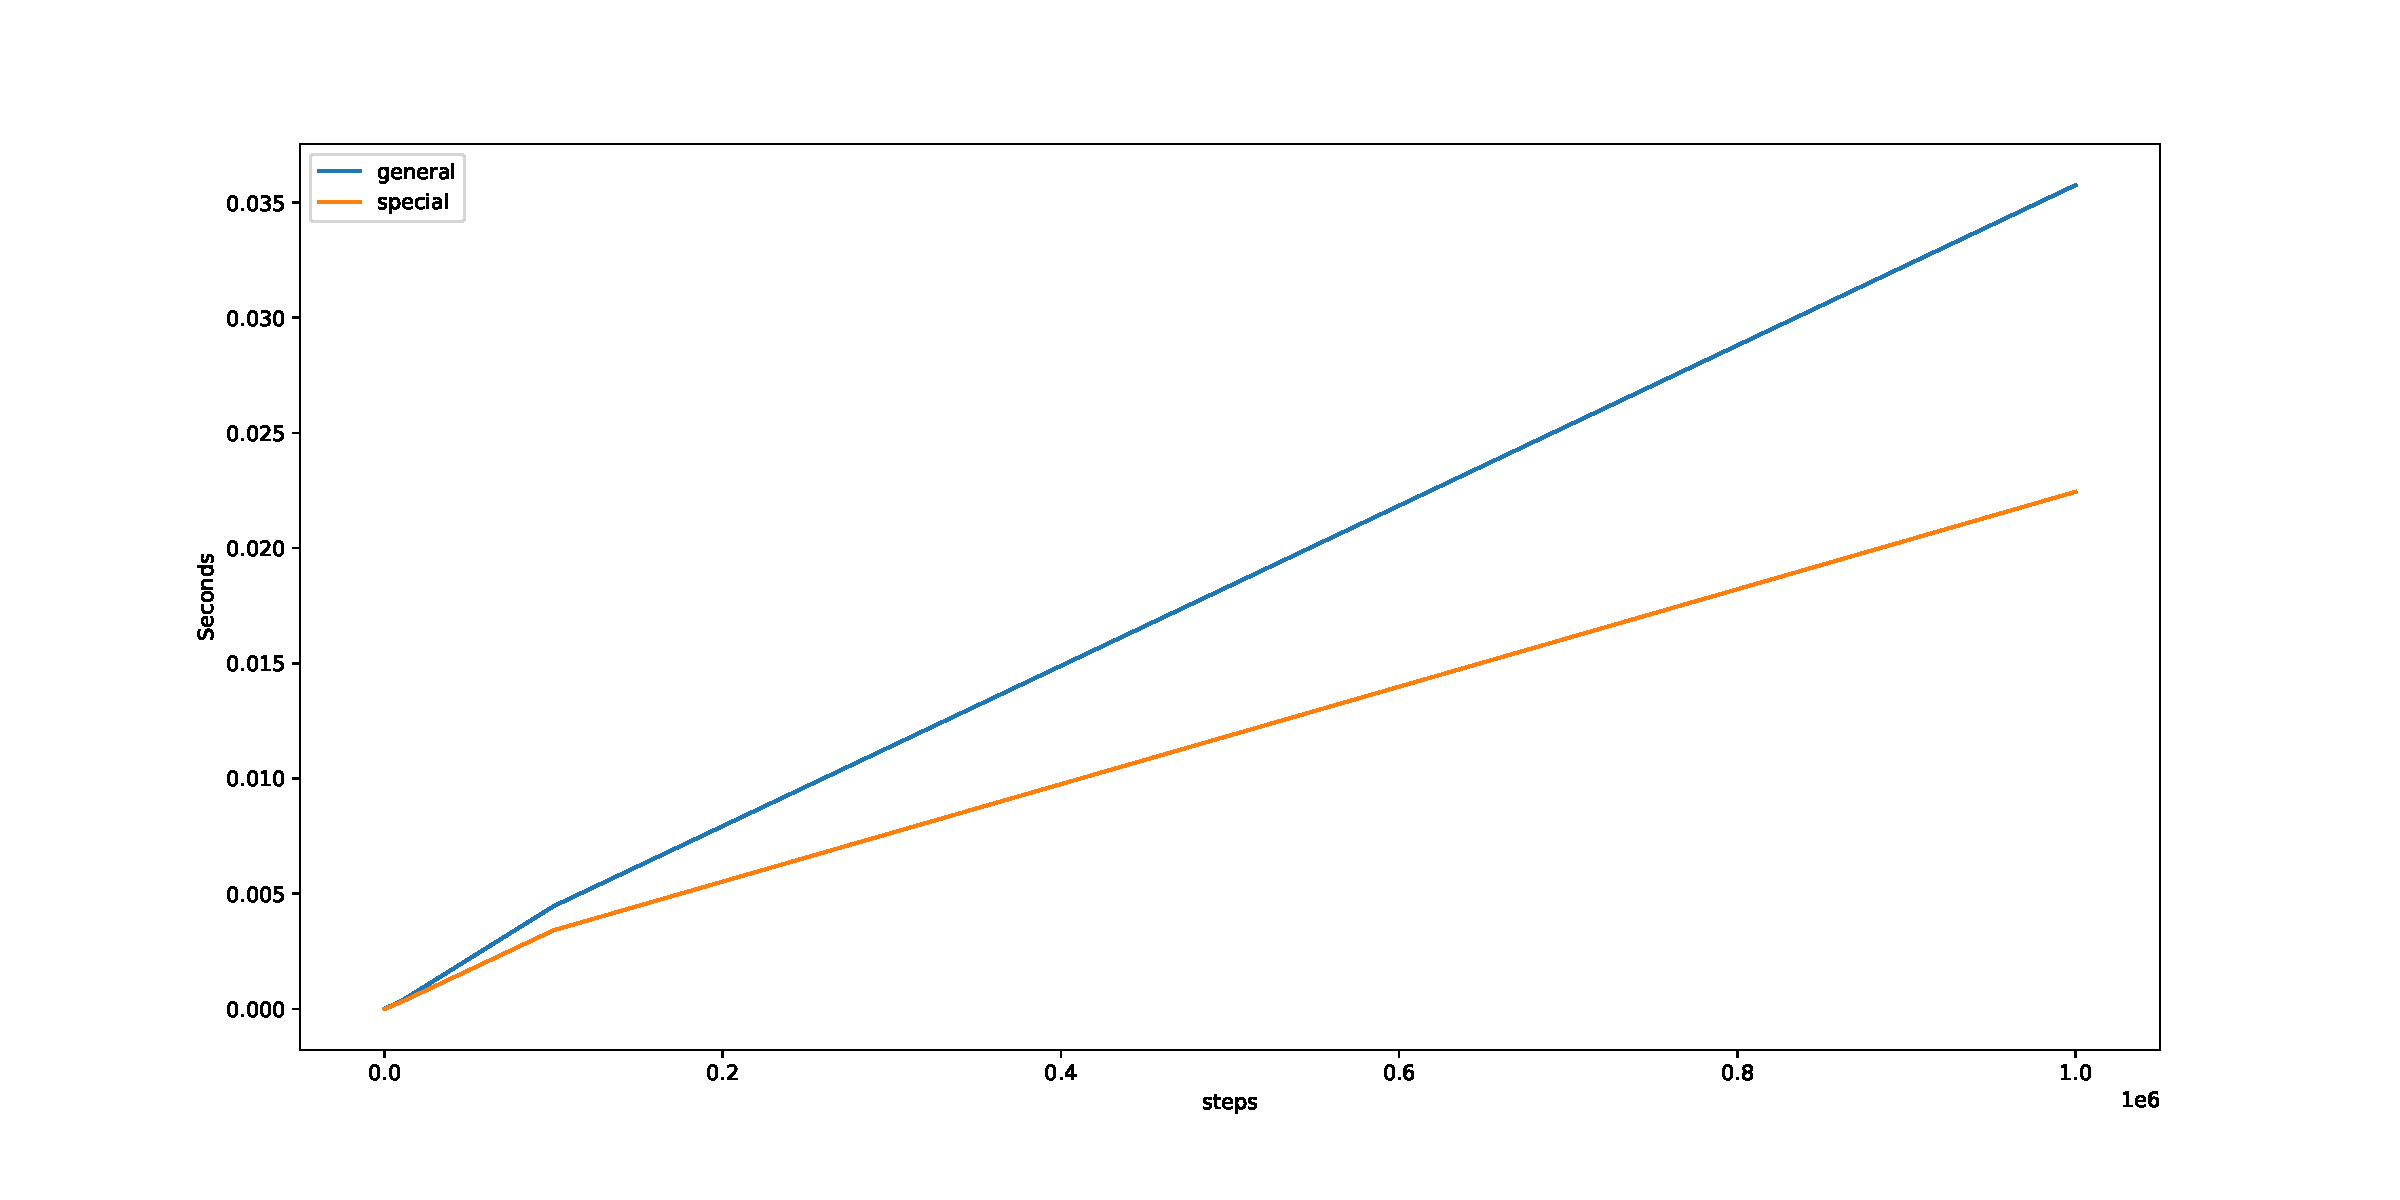
\includegraphics[scale=0.5]{../Figures/problem10.pdf}
	\caption{Numerical solution using the general algorithm with varying values of n vs the exact solution u(x)}
\end{figure}

\end{document}
